\section{Experiments}

We apply the developed methods to a variety of datasets, to show the power of the method across different scenarios. We choose datasets to span a range of node counts $N$, edge counts $E$ and feature space dimension $D$. We consider the following datasets:

\begin{itemize}
	\item \textbf{Political books} \cite{polbooks} ($N=105, E=441, D=3$) - network of Amazon book sales about U.S. politics, published close to the presidential election in 2004. Two books are connected if they were frequently co-purchased by the same customer. Vertex features encode the broad political affiliation of the author (liberal, conservative or neutral).
		
	\item \textbf{Primary school dynamic contacts} \cite{schools} ($N=238, E=5539, D=13$) - network of face-to-face contacts amongst students and teachers at a primary school in Lyon, France. Two nodes are connected if the two parties shared a face-to-face interaction over the course of the day. Vertex features include class membership, gender and whether or not the individual is a teacher or pupil. These data were collected on consecutive days in October 2009. We choose to analyse just the second day.
	
	\item \textbf{Facebook egonet} \cite{fb-snap} ($N=747, E=30025, D=480$) - an assortment of Facebook egonets. These are networks of a particular user's friends list and all the connections within that. Vertex features are extracted from each user's profile and are fully anonymized. We focus on the egonet with id 1912.
	
%	\item \textbf{Maier Facebook Egonet} \cite{FB-Maier}  ($N=349, E=2336, D=32$) - egonet of the author's Facebook friends list. Each vertex has been manually labelled with a variety of features describing their relationship to the author. For our purposes we remove all nodes of degree 1 (those that are only connected to the egonode) as these cannot be said to be part of any community present in the graph.
%		
%	\item \textbf{Law firm} \cite{LawFirm} - a network of relationships between members of a law firm. Each relationship is categorised according to type: coworkers, friends or advice.
%	
%	\item \textbf{Twitch users} \cite{twitch} - a network of user-user friendships on the streaming service Twitch. Vertex labels are extracted according to video-games played, location and streaming habits. This dataset is also broken down into disjoint networks according to language. We only consider the English users with is a subnet with $N=7126$ vertices and $E=35324$ edges).

\end{itemize}

We require metrics to assess the relative model evidence for the FFBM. This can be split into two separate components: the microcanonical SBM fit (concerned with the $b$-samples) and the fit of the feature-to-block generator (concerned with the $\theta$-samples). The SBM has been extensively analysed in other works \cite{Peixoto-Bayesian-Microcanonical} so that will not be the emphasis of our analysis. $S(b)$ (equation \ref{eqn:dl-form}) can be interpreted as the description length of the partition imposed by $b$. In other words this is the amount of information needed to describe the graph and the associated SBM parameters. It is only natural to divide this quantity by the number of entities (nodes and edges) in our graph $N+E$ to allow for rough comparison between graphs. We use a simple metric to gauge the fit of the SBM: the description length per entity averaged over the $b$-samples (equation \ref{eqn:mean-dl}):
%
\begin{equation}
	\bar{S}_e \coloneqq \frac{1}{(N+E) |\Tcal_b|} \sum_{t\in \Tcal_b} S \left( b^{(t)} \right)
	\label{eqn:mean-dl}
\end{equation}
%
However, to assess the performance of the feature-to-block predictor, we must partition the vertex set $[N]$ into training and test sets -- $\Gcal_0$ and $\Gcal_1$ respectively
\footnote{We choose to randomly create the partition on each experiment run such that a fraction $f$ of the available vertices form our training set $\Gcal$ and the remaining vertices are held out to form our test set $\Gcal^C$. For all the experiments $f=0.7$.}
. The $b$-chain is run using the whole network but we only use vertices $v \in \Gcal$ to train the $\theta$-chain. As $|\Gcal_0| \neq |\Gcal_1|$ sets, we cannot use the un-normalised log target $U$ (equation \ref{eqn:U-form}) for comparison between the two, as the prior term will be equal between the two but the total cross-entropy loss will be scaled by the size of each set. We therefore must use the average cross-entropy loss over each set (equation \ref{eqn:cross-entropy-loss}).
%
\begin{equation}
	\bar{\Lcal}_a \coloneqq \frac{1}{|\Tcal_\theta|} \sum_{t \in \Tcal_\theta} \Lcal_a \left( \theta^{(t)} \right)
	\qquad \textrm{where} \qquad
	\Lcal_a \left( \theta^{(t)} \right) \coloneqq \frac{1}{|\Gcal_a|} \sum_{i \in \Gcal_a}\sum_{j \in [B]} \hat{y}_{ij} \log \frac{1}{\phi_j \left(x_i; \theta^{(t)} \right)}
	\label{eqn:cross-entropy-loss}
\end{equation}
%
Where $a \in \{0, 1\}$ has been introduced to toggle between training and test sets. Table \ref{tab:results} summarises the results for each experiment. We run each experiment $n=10$ times with the same hyper-parameter values\footnote{For a comprehensive list of the hyper-parameters used for each experiment please see appendix \ref{appdx:hyperparams}} and report the mean plus or minus one standard deviation.

However, we also wish to determine the power of the dimensionality reduction method. For this we discard all features that satisfy equation \ref{eqn:discard}, to reduce the dimension from $D$ to $D'$. We then retrain the feature-block predictor using just the retained features and report the loss over the training and test sets for the reduced classifier -- denoted $\bar{\Lcal}_0'$ and $\bar{\Lcal}_1'$ respectively. These values are also included in the table except for the polbooks dataset as this is already very low.

\begin{table}[!h]
	\centering
	\caption{Results}
	\label{tab:results}
	\resizebox{\textwidth}{!}{%
	\begin{tabular}{c|ccc|c|cc|ccc}
		Dataset  & $B$ & $D$ & $D'$ & $\bar{S}_e$ & $\bar{\Lcal}_0$ & $\bar{\Lcal}_1$ & $c^*$ & $\bar{\Lcal}_0'$ & $\bar{\Lcal}_1'$  \\ \hline
		Polbooks & 3 & 3 & -- & $2.250 \pm 0.001$ & $0.584 \pm 0.033$ & $0.557 \pm 0.061$ & -- & -- & -- \\
		School & 10 & 13 & 10 & $1.894 \pm 0.006$ & $0.793 \pm 0.096$ & $0.914 \pm 0.112$ & $1.112 \pm 0.23$ & $0.791 \pm 0.096$ & $0.864 \pm 0.139$ \\
		FB egonet & 10  & 480 & 10 & $1.626 \pm 0.003$ & $1.305 \pm 0.034$ & $1.539 \pm 0.087$ & $0.942 \pm 0.042$ & $1.496 \pm 0.093$ & $1.578 \pm 0.104$
	\end{tabular}
	}
\end{table}

\FloatBarrier

\begin{figure}[!h]
	\centering
	\begin{subfigure}[t]{0.28\linewidth}
		\centering
		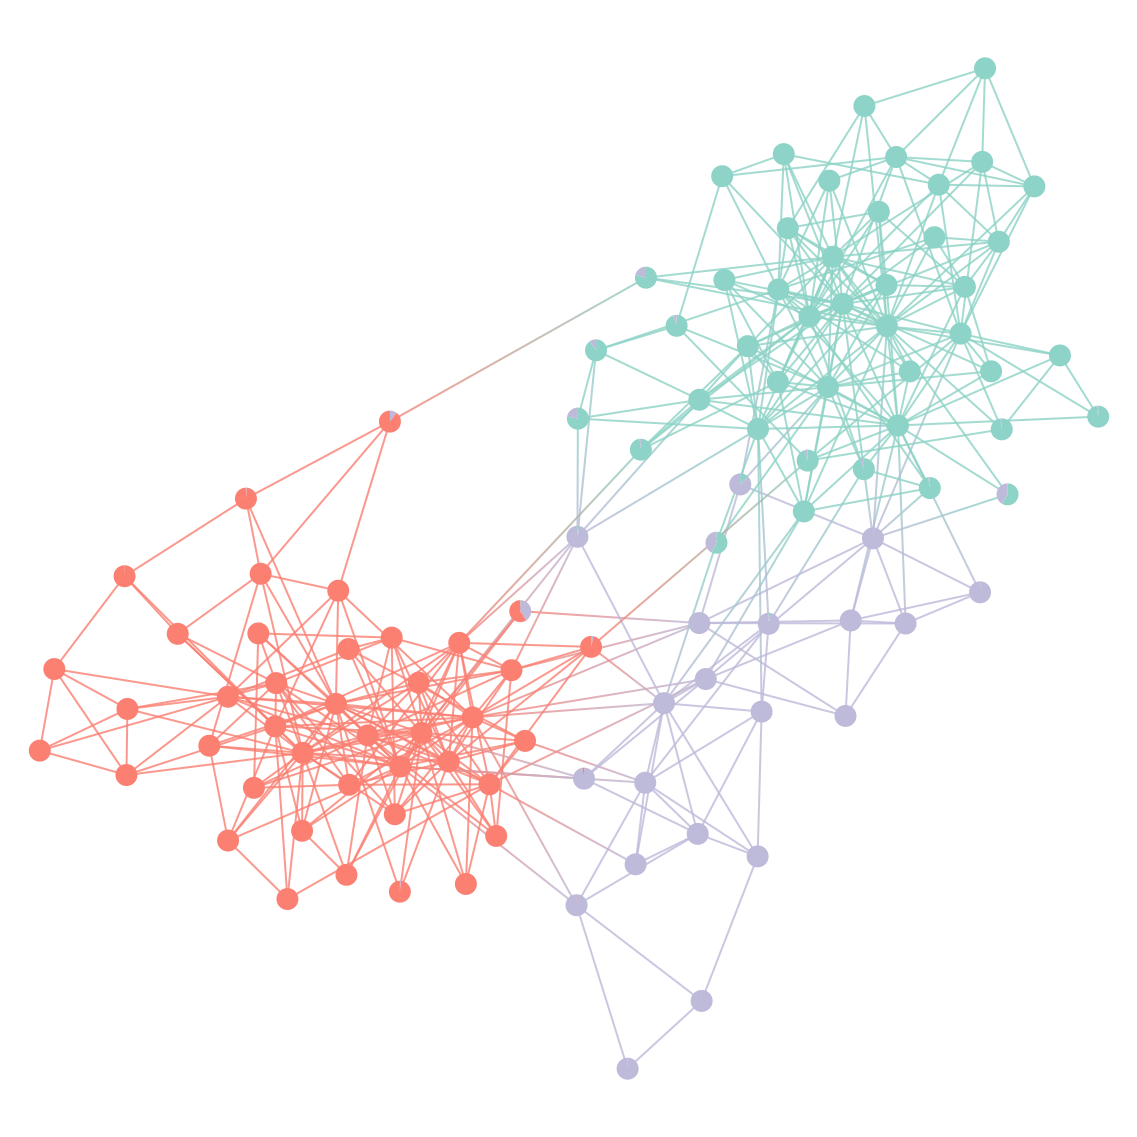
\includegraphics[width=\linewidth]{polbooks-graph.png}
		\caption{Polbooks}
		\label{fig:polbooks-graph}
	\end{subfigure}
	\hfill
	\begin{subfigure}[t]{0.28\linewidth}
		\centering
		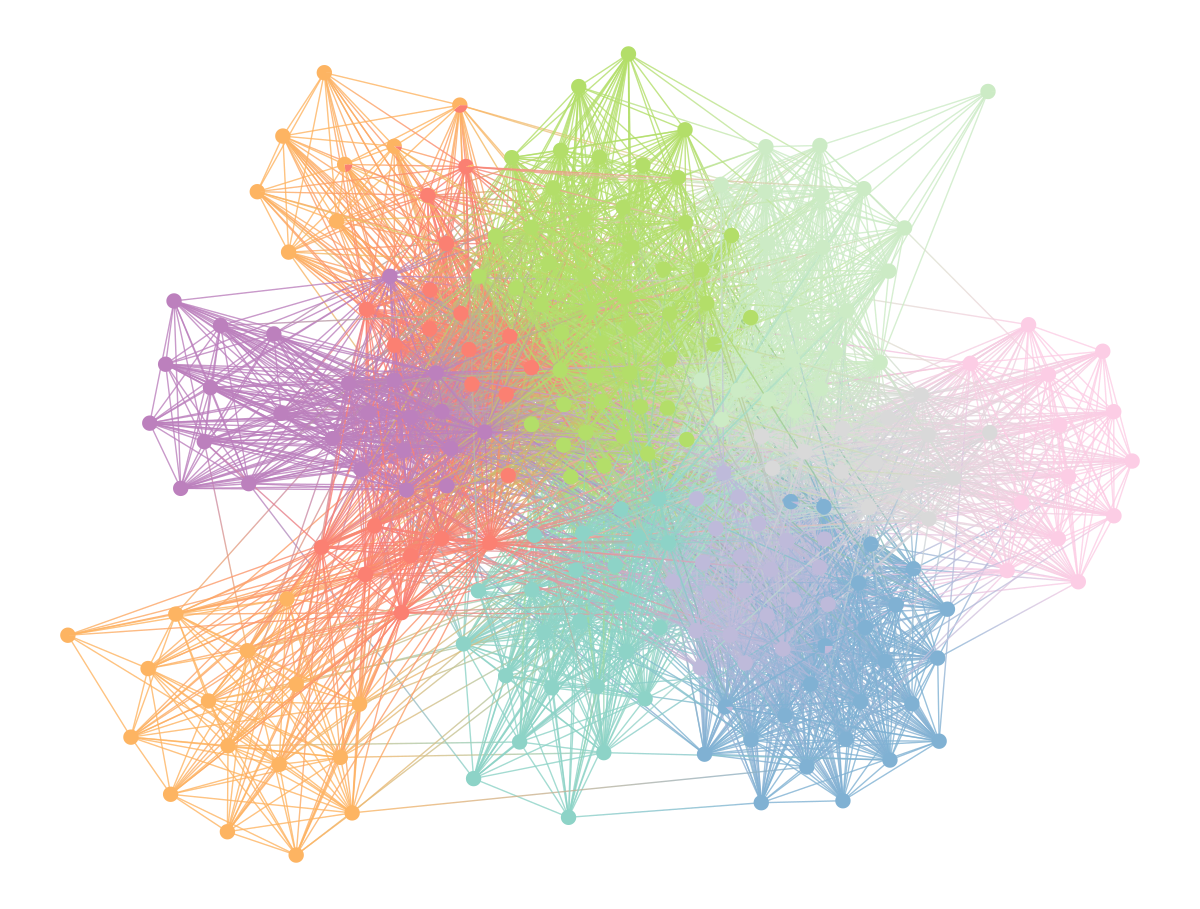
\includegraphics[width=\linewidth]{school-graph.png}
		\caption{School}
		\label{fig:school-graph}
	\end{subfigure}
	\hfill
	\begin{subfigure}[t]{0.28\linewidth}
		\centering
		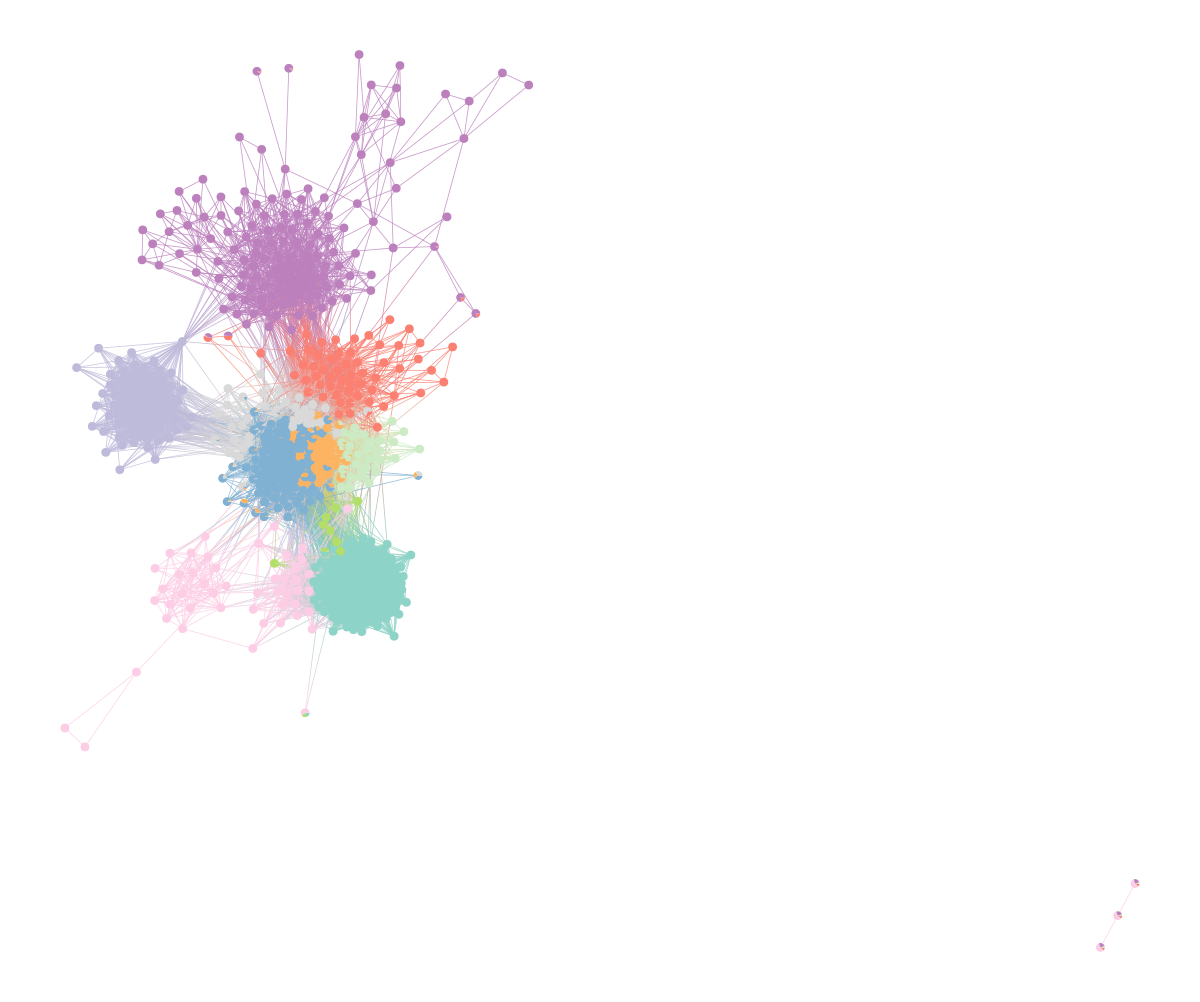
\includegraphics[width=\linewidth]{fb-graph.png}
		\caption{Facebook egonet}
		\label{fig:fb-graph}
	\end{subfigure}
	\begin{subfigure}[t]{0.10\linewidth}
		\centering
		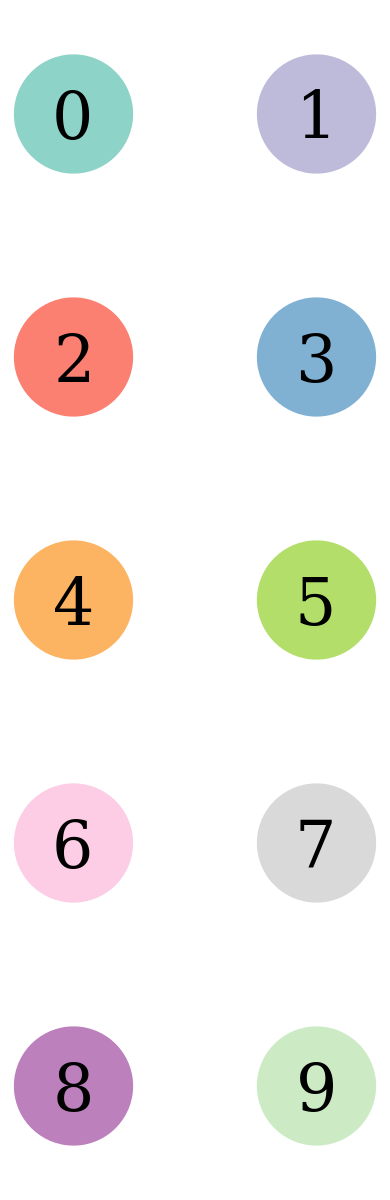
\includegraphics[width=0.8\linewidth]{10-vertical-legend.png}
		\caption{Legend}
		\label{fig:10-legend}
	\end{subfigure}
	\caption{Networks laid out and coloured according by inferred block memberships $\hat{y}$ for a given experiment iteration. Visualisation performed using \textit{graph-tool} \cite{peixoto_graph-tool_2014}}
\end{figure}


\begin{figure}[!h]
	\centering
	\begin{subfigure}[t]{0.32\linewidth}
		\centering
		\vskip 0pt
		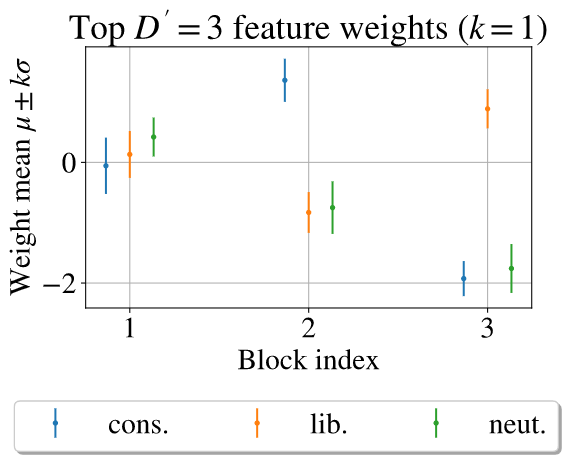
\includegraphics[width=\linewidth]{polbooks-null.png}
		\caption{Polbooks}
		\label{fig:polbooks-null}
	\end{subfigure}
	\hfill
	\begin{subfigure}[t]{0.32\linewidth}
		\centering
		\vskip 0pt
		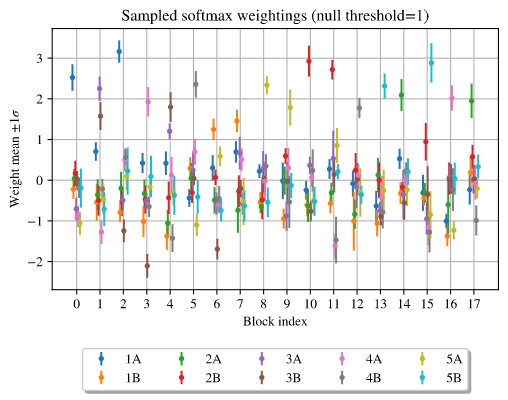
\includegraphics[width=\linewidth]{school-null.png}
		\caption{School}
		\label{fig:school-null}
	\end{subfigure}
	\hfill
	\begin{subfigure}[t]{0.32\linewidth}
		\centering
		\vskip 0pt
		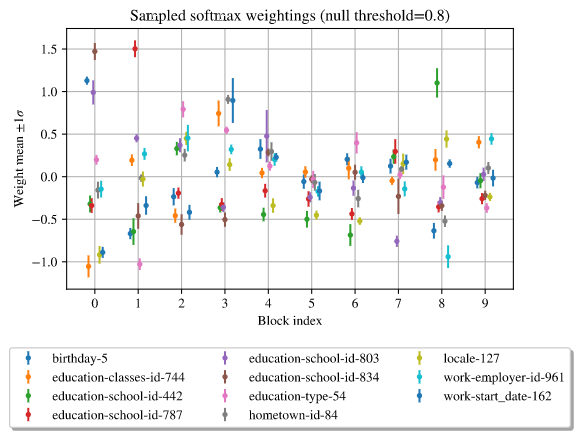
\includegraphics[width=\linewidth]{fb-null.png}
		\caption{Facebook egonet}
		\label{fig:fb-null}
	\end{subfigure}
	\caption{Reduced dimension feature-to-block generator weight samples}
\end{figure}

\subsection{Political books}

This dataset was collected by \citet{polbooks}. We wish to determine whether political affiliation is a good predictor of the overall network structure. We choose to partition the network into $B=3$ communities as we only have this many distinct values for political affiliation (conservative, liberal or neutral). The inferred block memberships are given in figure \ref{fig:books-graph}. We sample the block-generator parameters and plot the emprical mean and standard deviation of each sample on figure \ref{fig:book-null}.

Indeed, for all 3 blocks, each has a distinct political affiliation as its highest magnitude component. This is strong evidence that political affiliation is indeed the axis which best predicts the 3-way natural partition of the graph into blocks. Nevertheless, for block index 1, although \verb*|neutral| is the best predictor of the ones we have available, the value is not particularly extreme. Perhaps, there is an unobserved feature that places a book into this block. Indeed, block-0 is more of a centre-right block than true centre.

\FloatBarrier
\subsection{Primary school dynamic contacts}

These data were originally collected by \citet{schools} to quantify the transmission opportunities for respiratory infections. However, we seek to ask which vertex features best describe how people interact with one another in a primary school context. The only vertex features we have available are school-class (one of 10 values - 2 per year group), gender and a distinction between teachers and pupils.

We must first choose the number of blocks $B$ to define the coarseness of our analysis. A total of 10 school-classes would suggest that $B=10$ is a natural starting point. We visualise the inferred block memberships in figure \ref{fig:school-graph}.

As before, we proceed to sample the block-generator parameters $\theta$ and employ the dimensionality reduction heuristic defined in section \ref{sec:dim-reduction} with null threshold $c=1$ and standard deviation multiplier $k=1$. We then plot the weights for the features that survive the discard step in figure \ref{sec:dim-reduction}. Immediately, we see that only the pupils' class memberships have survived (1A-5B); gender and teacher/student status have been discarded meaning that these are not good predictors of overall macro-structure.

The vast majority of blocks are composed of a single class. However, some blocks have 2 comparably good classes as their predictor. For example, blocks 2 and 4 contain classes 4A and 4B as their 2 best predictors. This suggests that the social divide between classes is less pronounced for pupils in year 4 but there is nonetheless an unobserved variable that splits year 4 into 2 communities. The most surprising block is number 5 - which has comparable weightings for classes 5A and 1B. Perhaps there was a joint event between those two classes on the day the data were collected.

\subsection{Facebook egonet}

This dataset was chosen to showcase the power of the dimensionality reduction technique as the feature-space has high dimension ($D=480$). We sample the $b$-chain specifying $B=10$ total blocks and use this to construct the $\theta$-samples as before. 

We apply the dimensionality reduction heuristic outlined in section \ref{sec:dim-reduction}, choosing $k=1$ and $c=0.8$. This leads to a reduced dimension $D'=13$. These parameter values are plotted on figure \ref{fig:fb-null}. The features that remain are those that best explain the high-level community structure. More so than language, gender or surname - the school\footnote{This includes higher education institutes} you attend is the best explanatory variable for how the observed network's communities are partitioned at the highest level. 

Nevertheless, this example also highlights a weakness of the method for high-dimensional feature spaces. When the feature dimension is very large, it becomes increasingly likely that a particular feature may uniquely identify a small set of nodes. If these nodes are all part of the same community then the classifier will overfit for that particular parameter. The regularisation term imposed by the prior goes some way to alleviating this problem but we see in figure \ref{fig:fb-null} that the feature \verb*|birthday-5| has a very high weight as it relates to block 0. It might be possible to shift the feature values such that they take values in $\{-1, 1\}$ rather than $\{0, 1\}$ but this approach falls down when input features are mutually correlated. Indeed, for features with discrete values such as the class memberships (1A, 1B, 2A \dots 5B) it is preferred to keep $x_i \in \{0, 1\}^D$ as then each block can be readily accept more than one mutually exclusive feature-group (i.e. two school-classes are part of the same block).

